%%=============================================================================
%% Methodologie
%%=============================================================================

\chapter*{\IfLanguageName{dutch}{Proof of concept}{Proefafdruk}}
\label{ch:Proof of concept}

Het doel van dit hoofdstuk is om een idee te creëren van de omgeving waarin Cisco Identity Services Engine is geïmplementeerd. Hierbij is een uitgebreide uitleg over de elementen die aanwezig zijn binnen deze omgeving is terug te vinden in dit hoofdstuk. Ieder hardware apparaat is zorgvuldig beschreven, zo is o.a. informatie te vinden over de specificatie, de configuraties en de instellingen van de hardware componenten. Daarnaast werd ook de implementaties van de virtuele machines verder toegelicht.
\newline
\newline
Samen met al deze informatie zijn ook belangrijke schema’s terug te vinden die een visueel beeld geven over dit afgezonderd netwerk. 
Vervolgens is er de sectie die de enquête bespreekt. In deze sectie is voornamelijk informatie terug te vinden omtrent de enquête bevraging. 

\section{Cisco Identity Services Engine omgeving}

Voor de implementaties en testen van Cisco Identity Services Engine en zijn benodigde services, is er een omgeving vereist. Deze omgeving werd voorzien door een Belgische aanbieder van digitale televisie, breedband-internet, mobiele telefonie, enz. Deze Belgische aanbieder staat gekend als Telenet Group N.V. Implementaties en de testen van Cisco Identity Services Engine en zijn benodigde services is uitgewerkt in een Telenet thuisnetwerk.
\newline
Met als gevolg beschikt dit thuisnetwerk over een aantal Access Points en een Telenet Modem. De kabelverbinding die data verzend vanuit Telenet naar de modem in het thuisnetwerk is een coaxkabel. M.a.w. is het thuisnetwerk verbonden met het Wide Area Network(ook gekend als WAN) dankzij de Telenet's coaxkabel.
\newline
\newline
Om de essentiële componenten van dit thuisnetwerk te beschermen tegen breuk, is de implementatie verder uitgewerkt in een afgezonderd netwerkje. Dit wordt mogelijk gemaakt met behulp van een virtuele opensource router/firewall zoals Pfsense. Dit virtuele routerje dient als gateway voor de verschillende VLAN’s, waarbij het thuisnetwerk gebruikt zal worden als ‘uplink’ naar het internet. 

\subsection{Server VMware ESXi}
Het afgezonderd netwerkje bestaat uit een rack server waarop een viertal virtuele machines draaien. Deze virtuele machine zijn: Cisco Identity Service Engine, het virtuele routerje, genaamd Pfsense en twee  Windows Server 2019 datacenters machines. De creatie van deze virtuele machines wordt mogelijk gemaakt door VMware ESXi. VWware ESXi is een type-1 hypervisor van enterprise-klasse, ontwikkeld door VMware voor het inzetten en bedienen van virtuele machines. 
\newline
\newline
De ESXi server is geconfigureerd door het gebruik van een ‘bootable usb’. Deze bootable usb bevatte al nodige software om de server te voorzien met VMware ESXi. Vervolgens werd de server geconfigureerd met een aantal belangrijke settings, zoals het instellen van een IP adres, subnet mask, raid controller, enz.
\newline
\newline
Volgende settings zijn voorzien op deze ESXi server: 

\begin{itemize}
	\item IP adres: 192.168.0.183
	\item Subnet: 255.255.255.0
	\item Default gateway: 192.168.0.1
	\item raid controller: RAID 10
\end{itemize}

\begin{figure}[H]
	\centering
	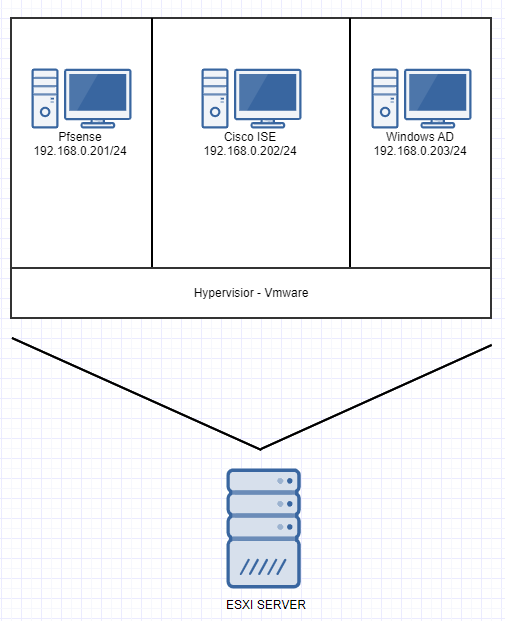
\includegraphics[height=0.3\textheight]{servervm.png}
	\caption{Deze afbeelding geeft een visueel beeld weer van de bestaande virtuele machines in de ESXi server.}
\end{figure}

\newpage
Door configuratie van deze IP instellingen, is de VMware ESXi toeganglijk via de webbrowser. Bovendien is de hard disk drive ingesteld als raid 10. Raid 10 is een hybride combinatie tussen raid 1 en raid 0. Waarbij men de snelheid van striping met de veiligheid van mirroring combineert. 
\newline
\newline
Dit is de veiligste en snelste methode maar ook de duurste. Het is een dure methode omdat er gebruik wordt gemaakt van raid 1, dus voor iedere 1TB aan opslagruimte is er ook 1TB aan mirror ruimte nodig, in combinatie met raid 0 waardoor er veel schijven nodig zijn. 

\begin{figure}[H]
	\centering
	\includegraphics[height=0.25\textheight]{Raid10.png}
	\caption{Deze afbeelding geeft een visueel beeld weer van een RAID 10 configuratie.}
\end{figure}

In deze server opstelling zijn drie van de vier fysieke ethernet adapters gebruikt. Deze adapters zijn op hun beurt verbonden met een virtuele switch. Elk van deze fysieke adapter heeft een andere functie. Deze functies zijn terug te vinden in onderstaande lijst. 

\begin{itemize}
	\item vmnic0,is de fysieke adapter die verbonden is met de virtuele switch, genaamd 'VSwitch0'.
	\item vmnic2,is de fysieke adapter die verbonden is met de virtuele switch, genaamd 'Sub\textunderscore switch'.
	\item vmnic3,is de fysieke adapter die verbonden is met de virtuele switch, genaamd 'Cisco \textunderscore switch'.
\end{itemize}

\newpage
\subsubsection{Virtuele switches}
\subsubitem{\bf VSwitch0}
\newline
De 'VSwitch0' is een virtuele switch die voorzien is om de VMware ESXi te contacteren via de webbrower. Deze switch is ingesteld met vlan id 0. Dit betekent m.a.w. dat hiervoor geen vlan identificatie is voorzien. 
\newline
\newline
Wanneer gebruikers surfen naar "https://192.168.0.183/", dan passeert deze data langs de fysieke poort vmnic0. Vervolgens stuurt de fysieke poort de data door naar de VSwitch0. Wanneer de data op de VSwitch0 terecht komt, stuurt hij op zijn beurt de data door naar de VMKernel poort.

\begin{figure}[H]
	\centering
	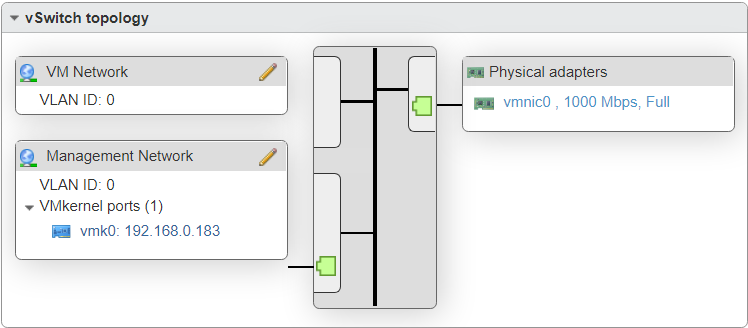
\includegraphics[width=0.7\textwidth]{VSwitch0.png}
	\caption{Deze afbeelding geeft een visueel beeld weer van de 'VSwitch0' topologie.}
\end{figure}

\subsubitem{\bf Sub\textunderscore switch}
\newline
De 'Sub\textunderscore switch' is een virtuele switch die gebruikt wordt als WAN interface voor de Pfsense. De WAN interface voorziet data overdracht van de thuis LAN netwerk naar het afgezonderd LAN netwerk. M.a.w. is connectie met het afgezonderd netwerkje mogelijk via deze interface. Bovendien is deze virtuele switch ook gebruikt voor de jumphost. Deze jumphost maakt het mogelijk om remote desktop protocol connecties te maken met de virtuele machines binnen het afgezonderd netwerkje. 
\newline
\newline
Vervolgens is deze virtuele switch ook ingesteld met vlan id 0. Dit betekend m.a.w. dat hiervoor geen vlan identificatie is voorzien. 

\begin{figure}[H]
	\centering
	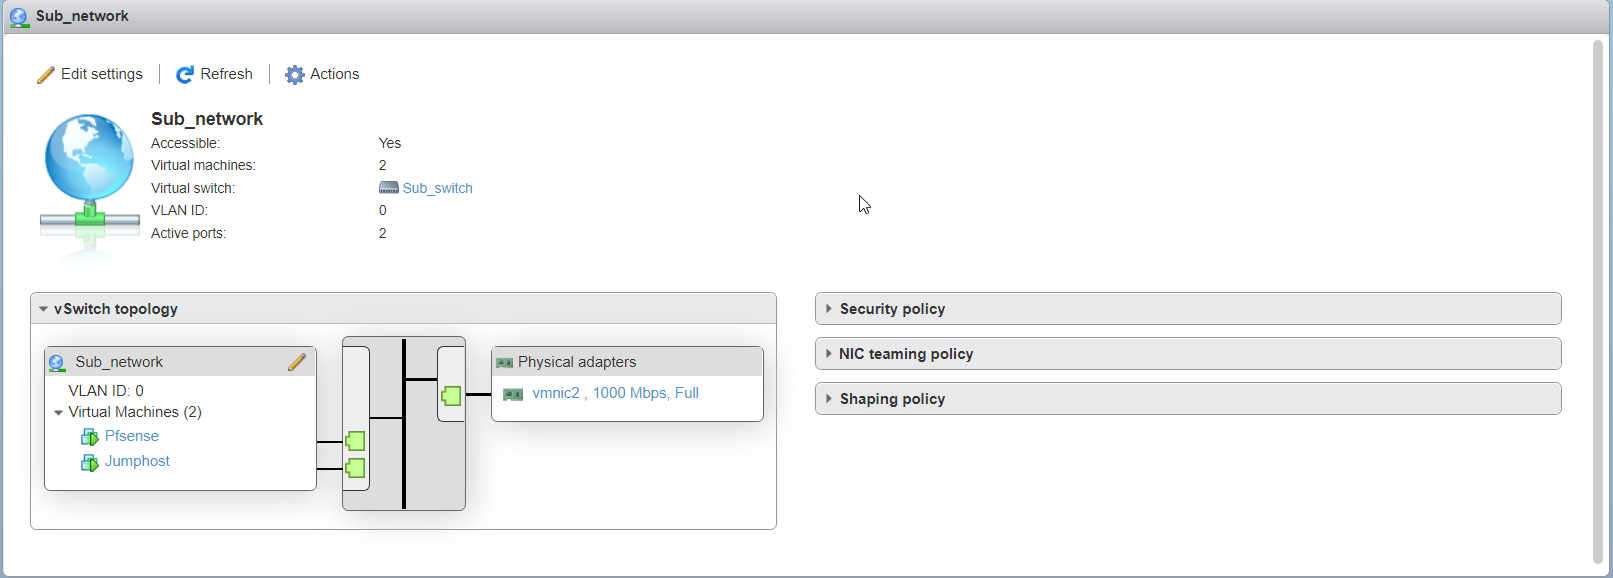
\includegraphics[width=0.7\textwidth]{Subswitch.png}
	\caption{Deze afbeelding geeft een visueel beeld weer van de 'Sub\textunderscore switch' topologie.}
\end{figure}

\subsubitem{\bf Cisco\textunderscore switch}
\newline
De 'Cisco\textunderscore switch'  is terug een virtuele switch. Deze switch wordt gebruikt om connectie te maken met alle apparaten achterliggend de fysieke Cisco switch. Dit betekent wanneer eind apparaten met de Cisco switch verbinden, dan zal de data passeren via deze virtuele switch. Bovendien bevinden alle andere virtuele machine zich in deze omgeving. Met als gevolgd is deze virtuele switch  ingesteld met vlan id 10. Dit betekent dat enkel data vanuit vlan 10 wordt doorgestuurd naar de voorziene machines.

\begin{figure}[H]
	\centering
	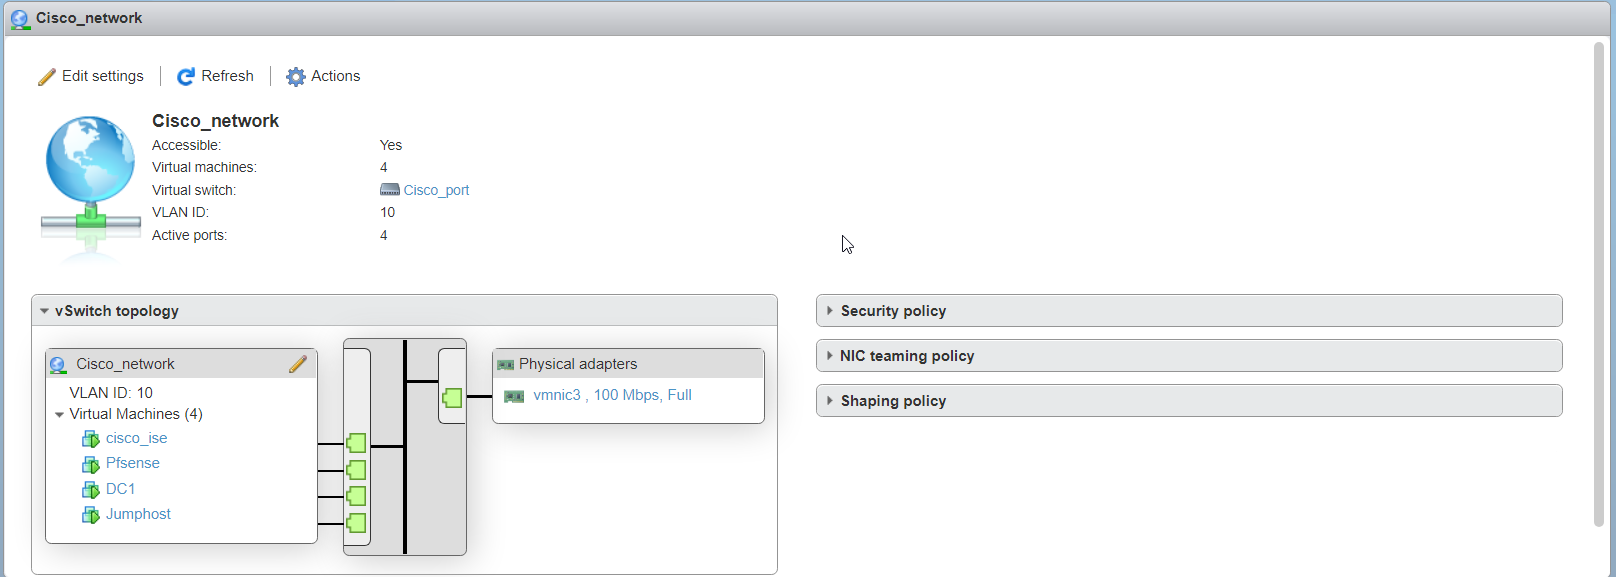
\includegraphics[width=0.7\textwidth]{CiscoSwitch_vmware.png}
	\caption{Deze afbeelding geeft een visueel beeld weer van de 'Cisco\textunderscore switch' topologie.}
\end{figure}

\subsubsection{Server ESXi specificaties}
De voorziene ESXi server is van het merk International Business Machines Corporation, gekend als IBM. Deze server werd oorsprongelijk gebruikt in de productie omgeving van Axians, maar is sinds kort een test server. 
\newline
\newline
Hierbij heeft ‘System x3350 M3’, gekend binnen Axians als ‘de oude shr-esx-04 server’, de volgende specificaties:

\begin{itemize}
	\item Vormfactor: 1U Rack
	\item Processor:
	\begin{itemize}
		\item Proccessorsnelheid: 2.53GHz
		\item Processor: 6-core processor
	\end{itemize}
	\item Geheugen:
	\begin{itemize}
		\item Intern geheugen: 240 GB Random Access Memory
		\item Intern geheugentype: Double Data Rate 3 Synchronous Dynamic Random-Access Memory, gekend als DDR3 SDRAM
	\end{itemize}
	\item Opslag:
	\begin{itemize}
		\item Maximum aantal schrijven: 8 Slots
		\item Opslag: 4 Terabyte HHD 7500 RPM
	\end{itemize}
	\item Netwerk
	\begin{itemize}
		\item Ethernet interface type: Gigabit Ethernet
		\item Aantal ethernet poorten: 4 
	\end{itemize}
\end{itemize}

\begin{figure}[H]
	\centering
	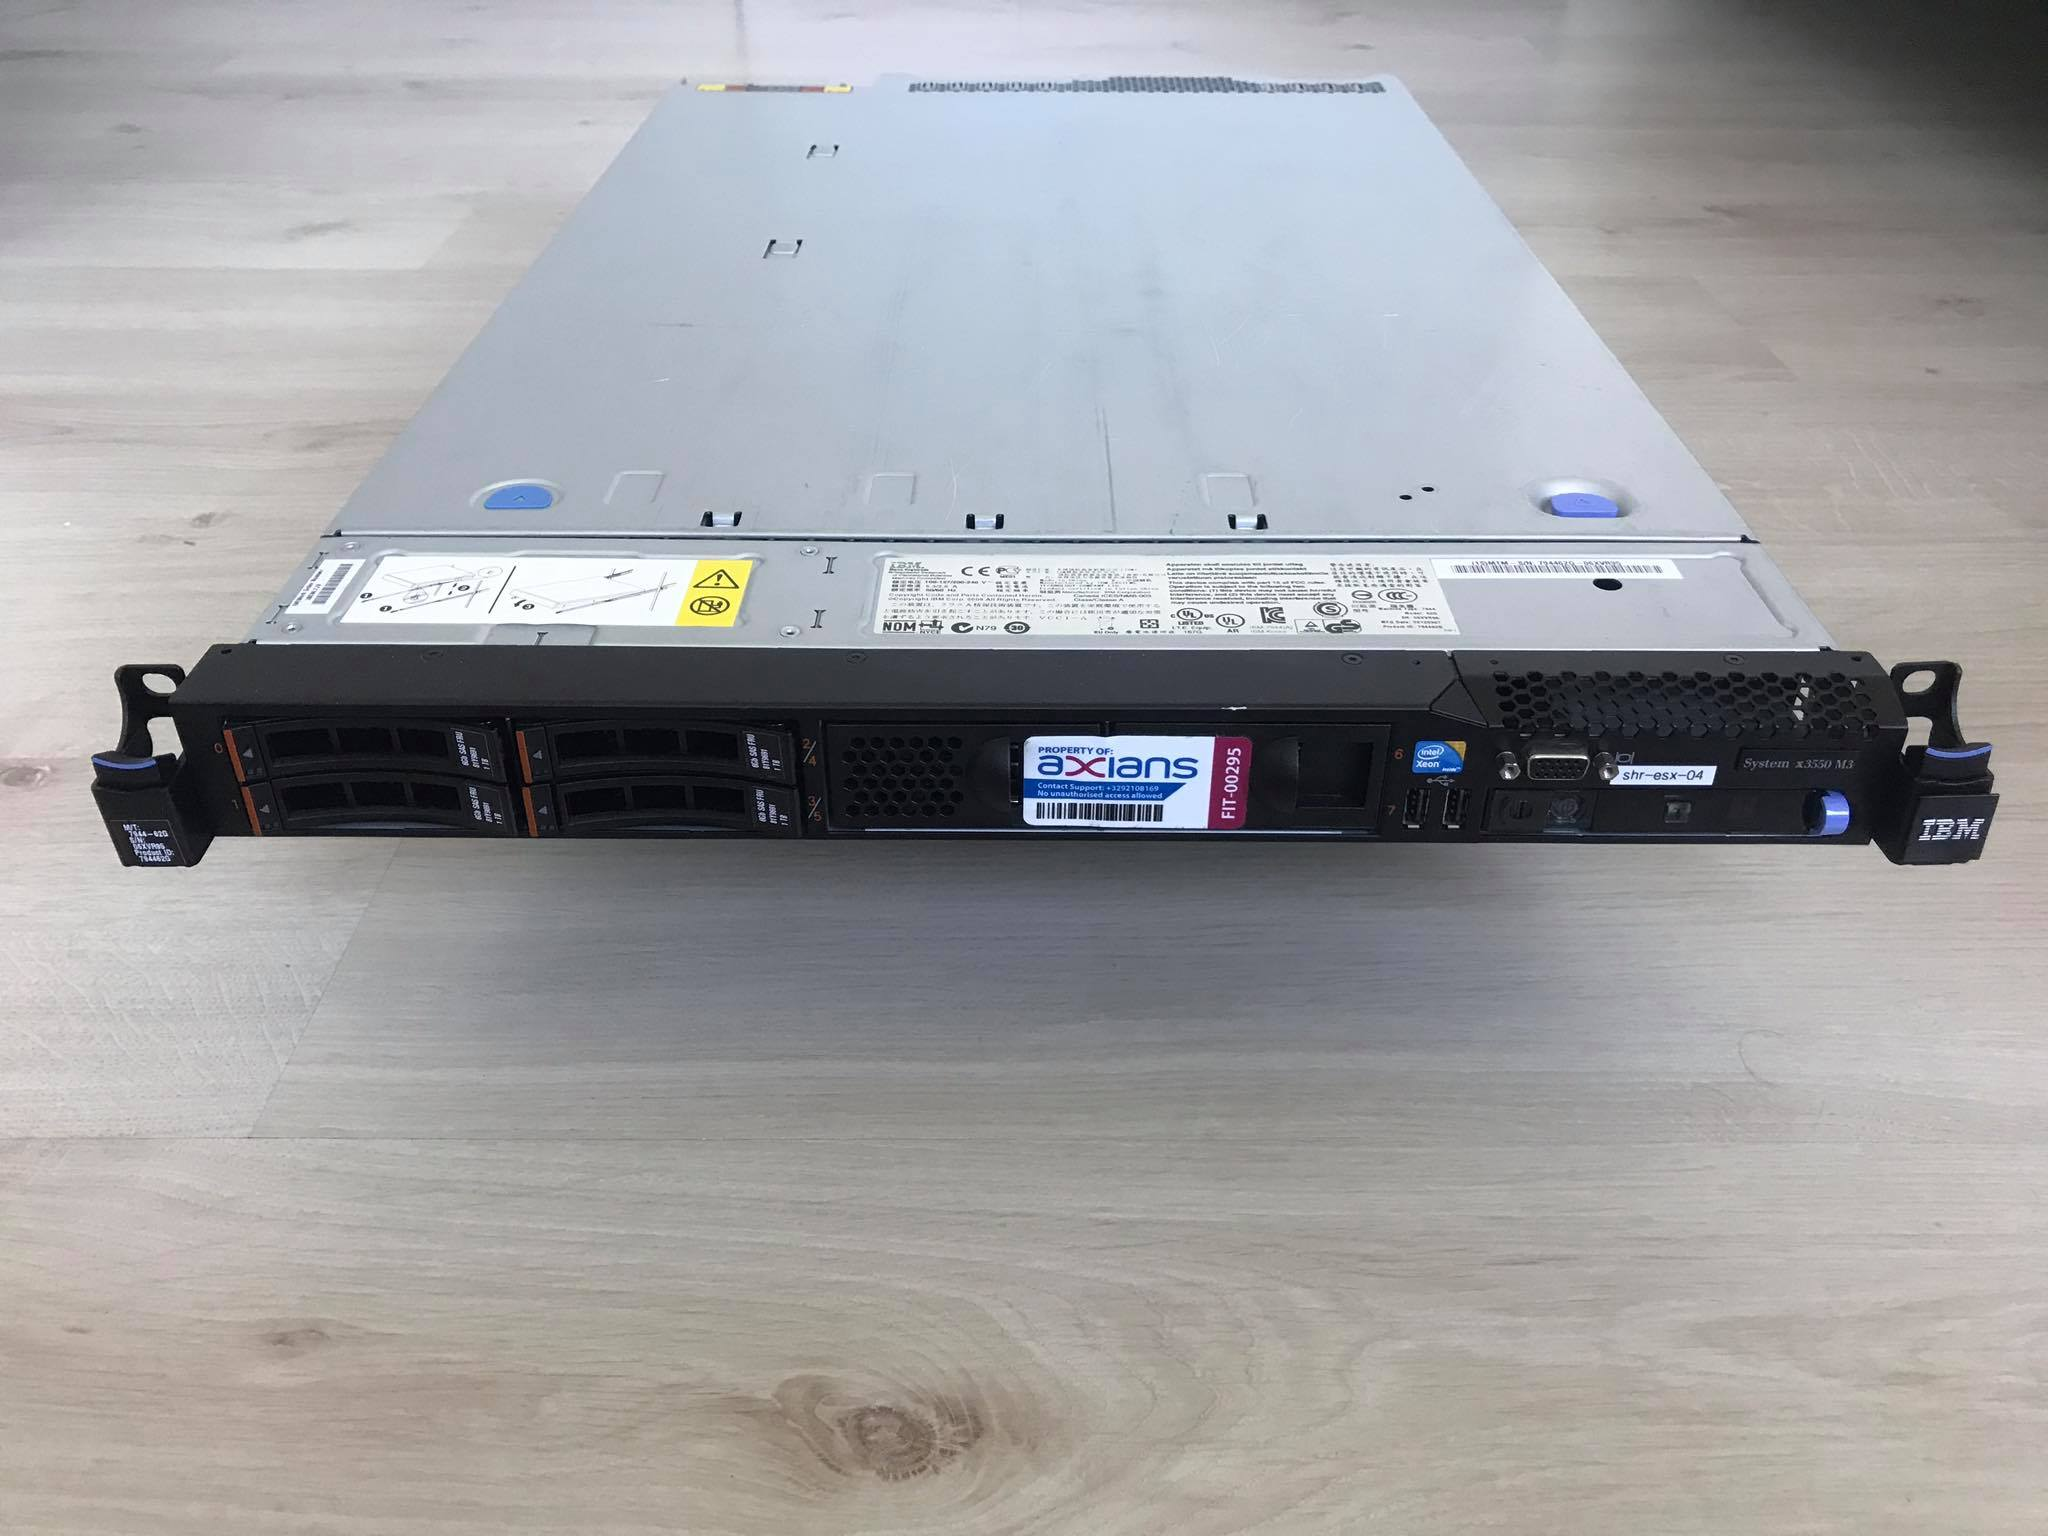
\includegraphics[width=0.5\textwidth]{serveresxi.png}
	\caption{Deze afbeelding heeft de ESXI server weer. }
\end{figure}

\subsection{Cisco switch}
Naast de ESXi server, bestaat de Cisco Identity Services Engine omgeving ook uit een Cisco switch. Deze fysieke switch werd geconfigureerd, zodanig dat de Cisco Identity Services Engine virtuele machine kan communiceren met deze switch. Om deze communicatie mogelijk te maken, zijn er bepaalde configuraties uitgevoerd op deze fysieke switch. Deze noodzakelijke configuraties speelden een belangrijke rol in de configuratie van de 'Port-based network access control' use case. 
\newline
\newline
Daarnaast zijn er ook een aantal basis configuraties uitgevoerd op deze switch. Hierdoor wordt communicatie tussen het afgezonderd netwerk en de eind apparaten achterliggend de switch ook mogelijk. Deze informatie is terug te vinden in de volgende subsectie.  

\subsubsection{Configuratie}
Om te beginnen werd de Cisco switch met een aantal commando's geconfigureerd. Deze configuraties beveiligen het network apparaat. M.a.w. zijn secrets, line password en passwords enqryption commando's uitvoert om inbreuk tegen te gaan. 
\newline
\newline
Om te communiceren met het afgezonderd netwerk, werd Gigabit Ethernet 0/1 geconfigureerd met volgende settings: 

\begin{itemize}
	\item switchport mode trunk
	\item switchport trunk allow vlan 10 
\end{itemize}

Deze configuratie maakt data overdracht van de verschillende vlan's mogelijk. Deze poort werd rechtsverbonden met één van de interfaces op de ESXi server. Vervolgens werd een vlan gecreeërt en kreeg het ip adres '192.168.17.5' met subnet mask '255.255.255.0' toegewezen. Deze instellingen behoorde tot de basis configuratie van de Cisco switch.

\begin{figure}[H]
	\centering
	\subfloat{{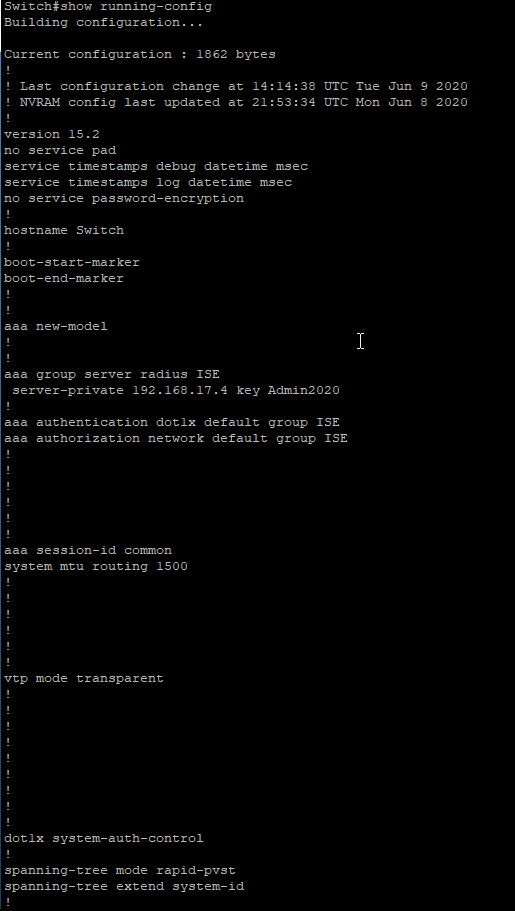
\includegraphics[width=3cm]{Switch_config1.png} }}%
	\qquad
	\subfloat{{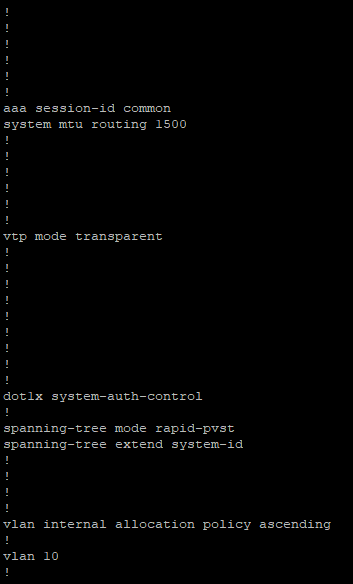
\includegraphics[width=3cm]{Switch_config2.png} }}%
	\qquad
	\subfloat{{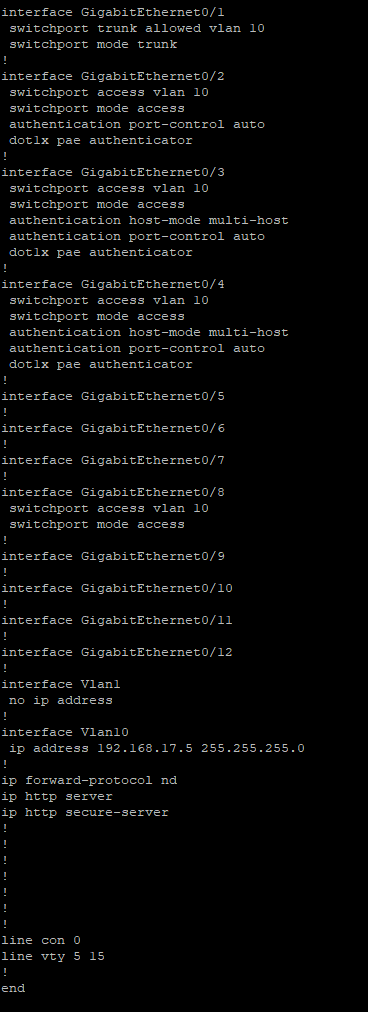
\includegraphics[width=3cm]{Switch_config3.png} }}%
	\caption{Bovenstaande foto's geven de running-config van de Cisco switch weer. Waarbij een aantal interfaces geconfigureerd zijn met het 'Policy-based network access control' use case.}%
	\label{fig:RunningConfig}%
\end{figure}

Vermits poort Gigabit Ethernet 0/1 geconfigureerd is om verbinding te maken met de server ESXi, zijn de overige poorten bedoeld voor de communicatie met de eind apparaten. Met als gevolg dat alle overige poorten ingesteld zijn met het 'Port-based network access control' use case.
\newline
\newline
Om de 'Port-based network access control' use case mogelijk te maken, werd een nieuw AAA model ingesteld. Vervolgens werd dit AAA model met een radius server geïnitialiseerd. De dot1x aaa authentication methode werd met zijn standaard netwerk group mee configureerd. 
\newline
\newline
Dot1x system-auth-control werd hierbij mee vastgelegd. Om de configuratie te beëindeigen, werden alle poorten voorzien van de nodige 'Port-based NAC' configuraties. Deze configuraties zijn in de volgende lijst weergegeven.

\begin{itemize}
	\item \#enable
	\item \#config t
	\item (config)\#aaa new-model
	\item (config)\#aaa group server radius ISE
	\item (config-sg-radius)\#server-private 192.168.17.4 key Admin2020
	\item (config-sg-radius)\#exit
	\item (config)\#aaa authentication dot1x
	\item (config)\#aaa authorization network default group ISE
	\item (config)\#dot1x system-auth-control
	\item (config)\#interface range gig0/2-12
	\item (config-if-range)\#switchport mode access
	\item (config-if-range)\#switchmode access vlan 10
	\item (config-if-range)\#authentication host-mode multi-host
	\item (config-if-range)\#authentication port-control auto
	\item (config-if-range)\#dot1x pae auth
	\item (config-if-range)\#end
\end{itemize}

\subsubsection{Communicatie}
Om deze systemen met elkaar te laten communiceren, werden 1G cat5e ethernet kabels gebruikt. Deze Unshielded Twisted Pair Ethernet kabels halen snelheden tot 1000 Mbit/s met een doorvoersnelheid van 100mhz. Wat geschikt is voor dit afgezonderd netwerk.

\subsubsection{Cisco switch specificaties}
Deze switch is van het merk Cisco Systems, en behoord tot de ‘Catalyst 2960-CX’ series. Deze Cisco switch staat nu gekend binnen Axians als de ‘Demo switch’. 
In onderstaande lijst vindt u de specificaties van de Cisco Catalyst 2960-CX serie switch:

\begin{itemize}
	\item Power over Ethernet:
	\begin{itemize}
		\item Ondersteunend: Ja
		\item Standaard: 802.3at (PoE+)
	\end{itemize}
	\item Netwerk:
	\begin{itemize}
		\item 8 Gigabit Ethernet aansluitingen
		\item 2 Gigabit Ethernet Copper uplinks
		\item 2 Gigabit Ethernet Small form-factor pluggable uplinks, gekend als SFP
	\end{itemize}
	\item Besturingsysteem/software:
	\begin{itemize}
		\item OS: Cisco IOS
\end{itemize}

\begin{figure}[H]
	\centering
	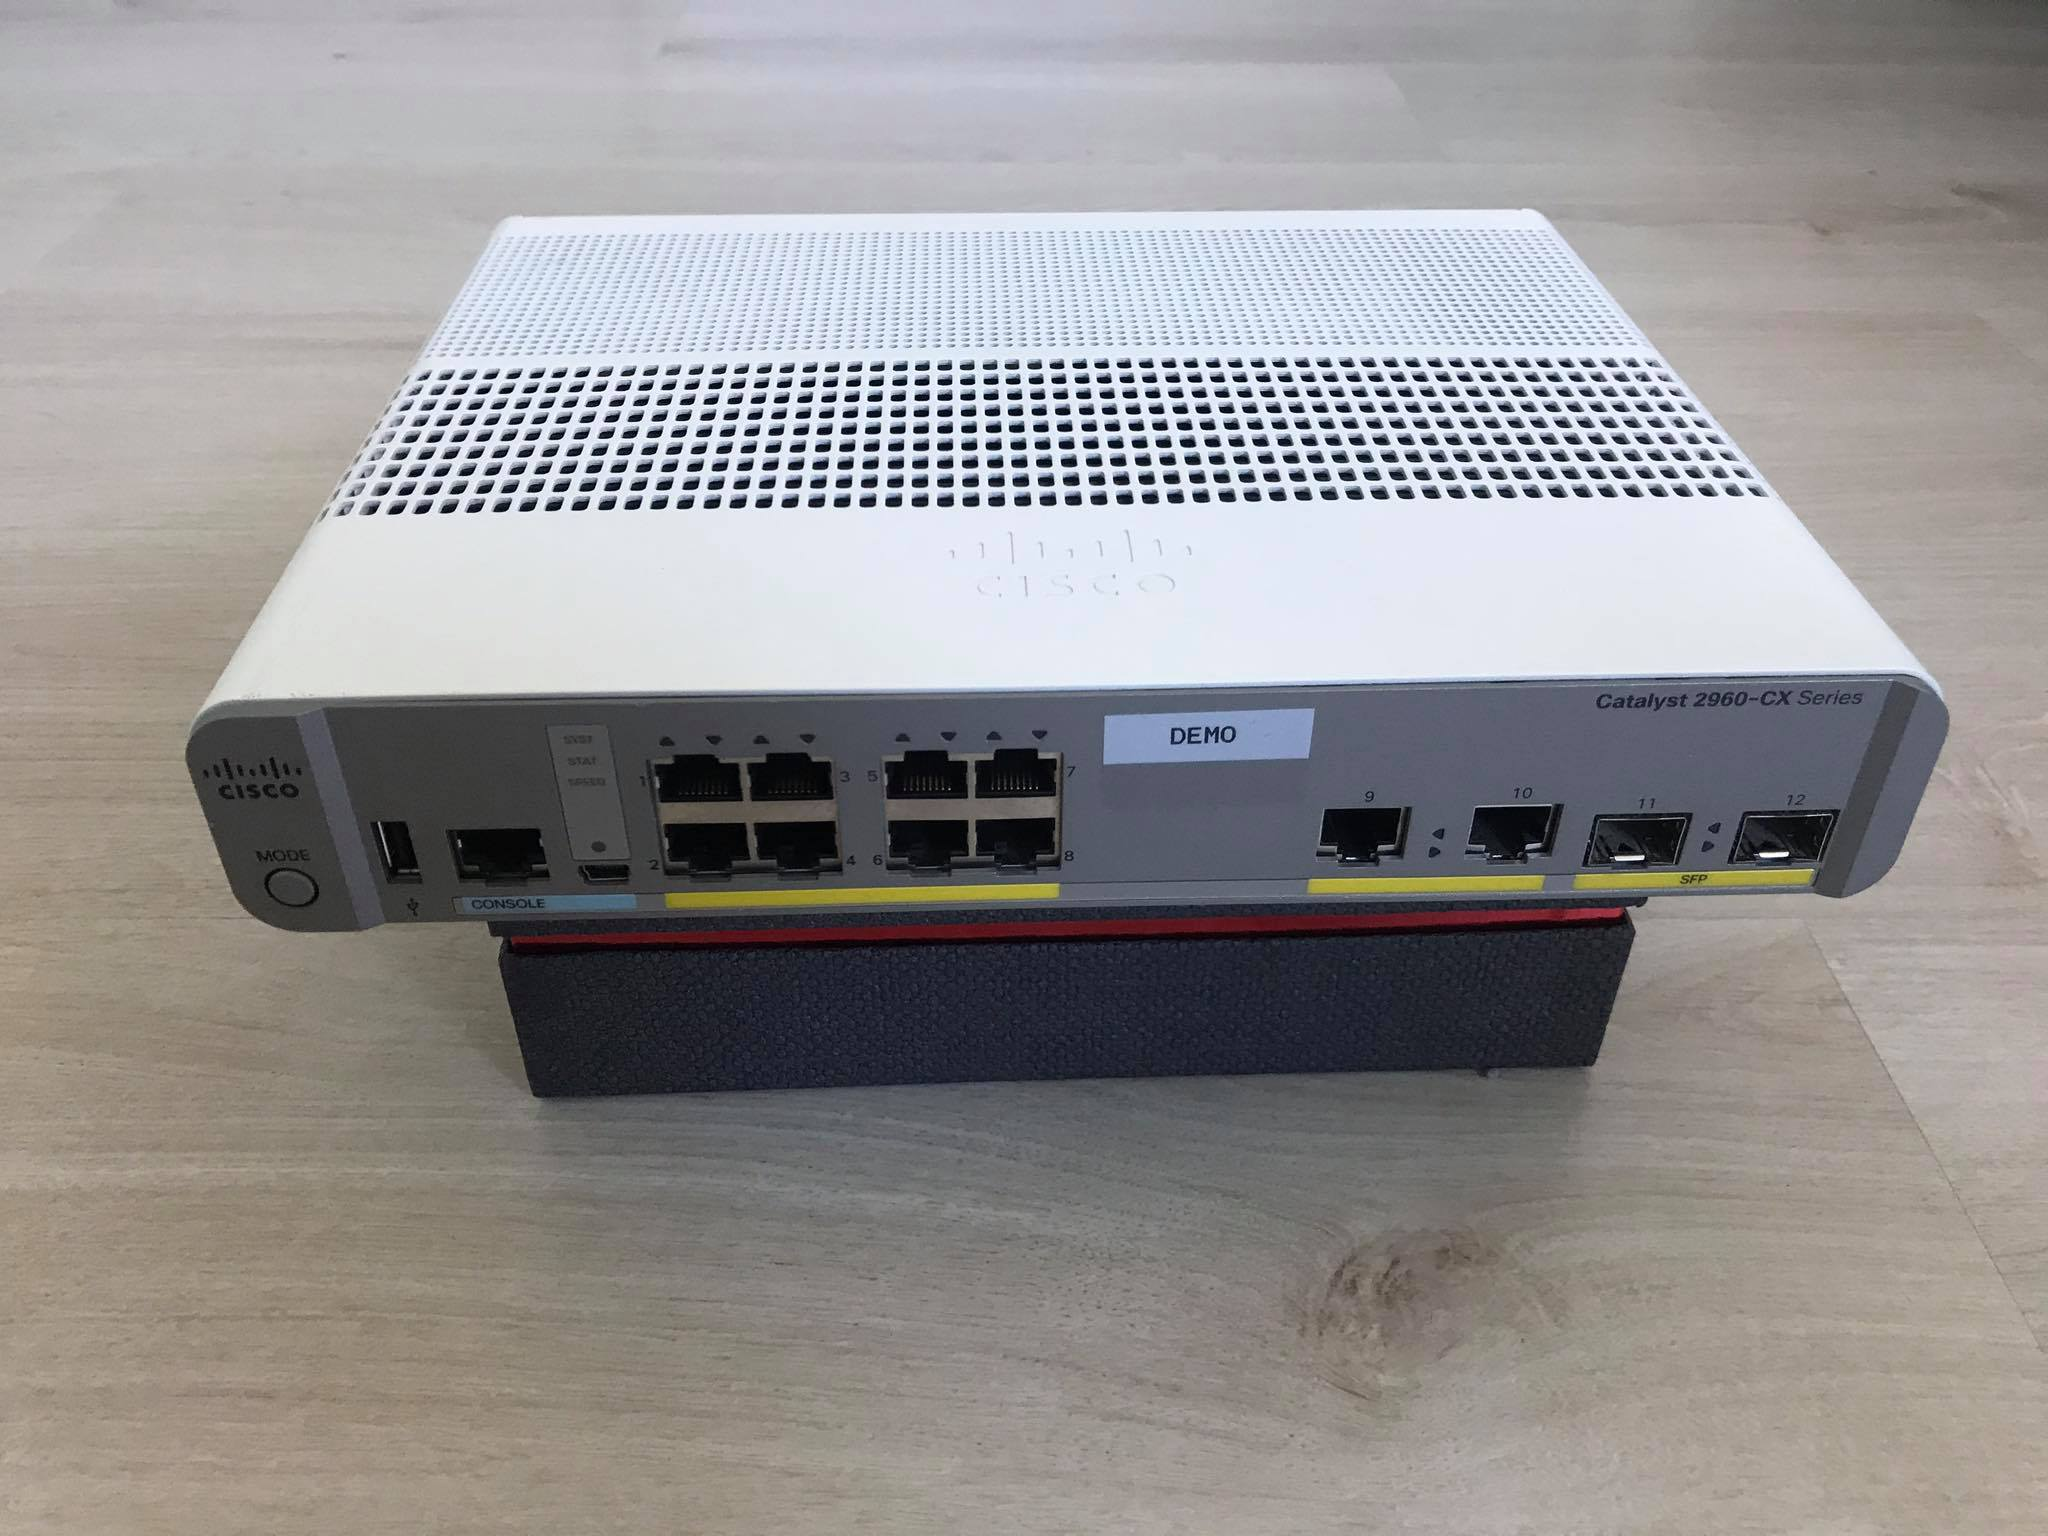
\includegraphics[width=0.5\textwidth]{ciscoswitch.png}
	\caption{Deze afbeelding heeft de Cisco switch weer. }
\end{figure}

\subsection{Virtuele machines}
\subsubsection{Cisco Identity Services Engine}
 TO DO! Praten over de omgeving en use case omgeving 
 \subsubitem{Port-based network access control}
 \subsubitem{Policy-based network access control}
 \subsubitem{Thread-centric network access control}
\newline
\newline

Dit systeem werd geïnstalleerd op een Red Hat Enterprise 7 distributie, waar vogende specificaties voor werd vrijgemaakt: 

\begin{itemize}
	\item Geheugen: 128 GB Random Access Memory
	\item Opslag: 512 GB
	\item CPU: 24 cores
	\item Netwerk adapter: Cisco\textunderscore netwerk
\end{itemize}

De installatie van Cisco Identity Services Engine werd mogelijk gemaakt door \cite{CiscoISE_InstallationGuide}.

\begin{figure}[H]
	\centering
	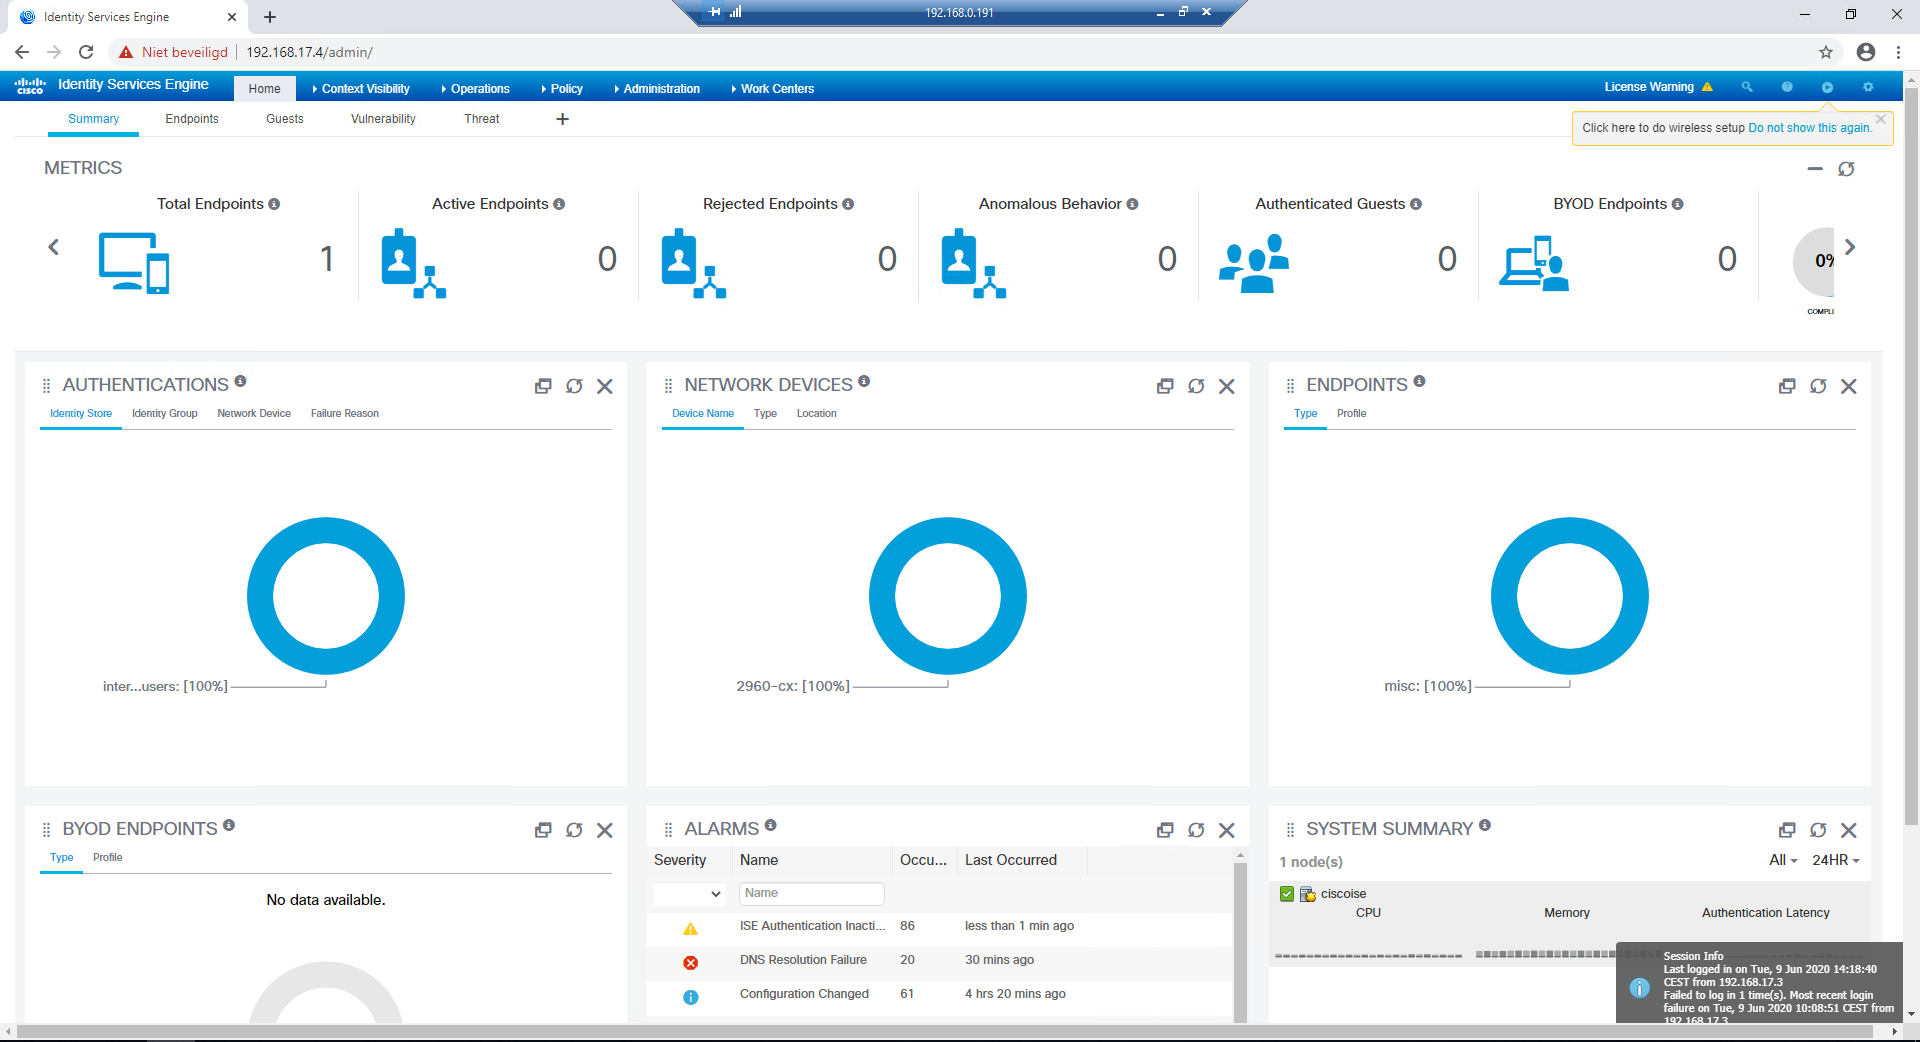
\includegraphics[width=0.5\textwidth]{homepage_ise.png}
	\caption{Deze afbeelding heeft de home page van Cisco Identity Services Engine weer.}
\end{figure}

\subsubsection{Windows server 2019 datacenter}
Op de windows server 2019 werd een Active Directory domain aangemaakt. Hiervoor werd een nieuwe forrest aangemaakt, genaamd ‘Bachelorproef.com’. Vervolgens werd deze server ook gepromoveerd naar de domaincontroller binnen het netwerk.
\newline
\newline
Via Cisco Identity Service Engine kan men subset van domeinen selecteren vanuit de vertrouwde domeinen voor authenticatie en autorisatie. Deze subset van domeinen worden authenticatiedomeinen genoemd. Het definiëren van deze authenticatiedomeinen verbetert de beveiliging door bepaalde domeinen te blokkeren, waardoor de authenticatie van de gebruikers op deze domeinen wordt beperkt.
\newline
\newline
Om dit systeem te contacteren, werd het ‘Remote Desktop Protocol (RDP)’ gebruikt met het Internet Protocol (IP) adres van dit systeem.
\newline
\newline
Dit systeem werd geïnstalleerd op een Microsoft omgeving, waar volgende specificaties voor werden vrijgemaakt:

\begin{itemize}
	\item Geheugen: 16 GB Random Access Memory
	\item Opslag: 126 GB
	\item CPU: 20 cores
	\item Netwerk adapter: Cisco\textunderscore netwerk
\end{itemize}
De installatie van Windows Server 2019 datacenter werd mogelijk gemaakt door \cite{Win19_InstallationGuide}. 

\begin{figure}[H]
	\centering
	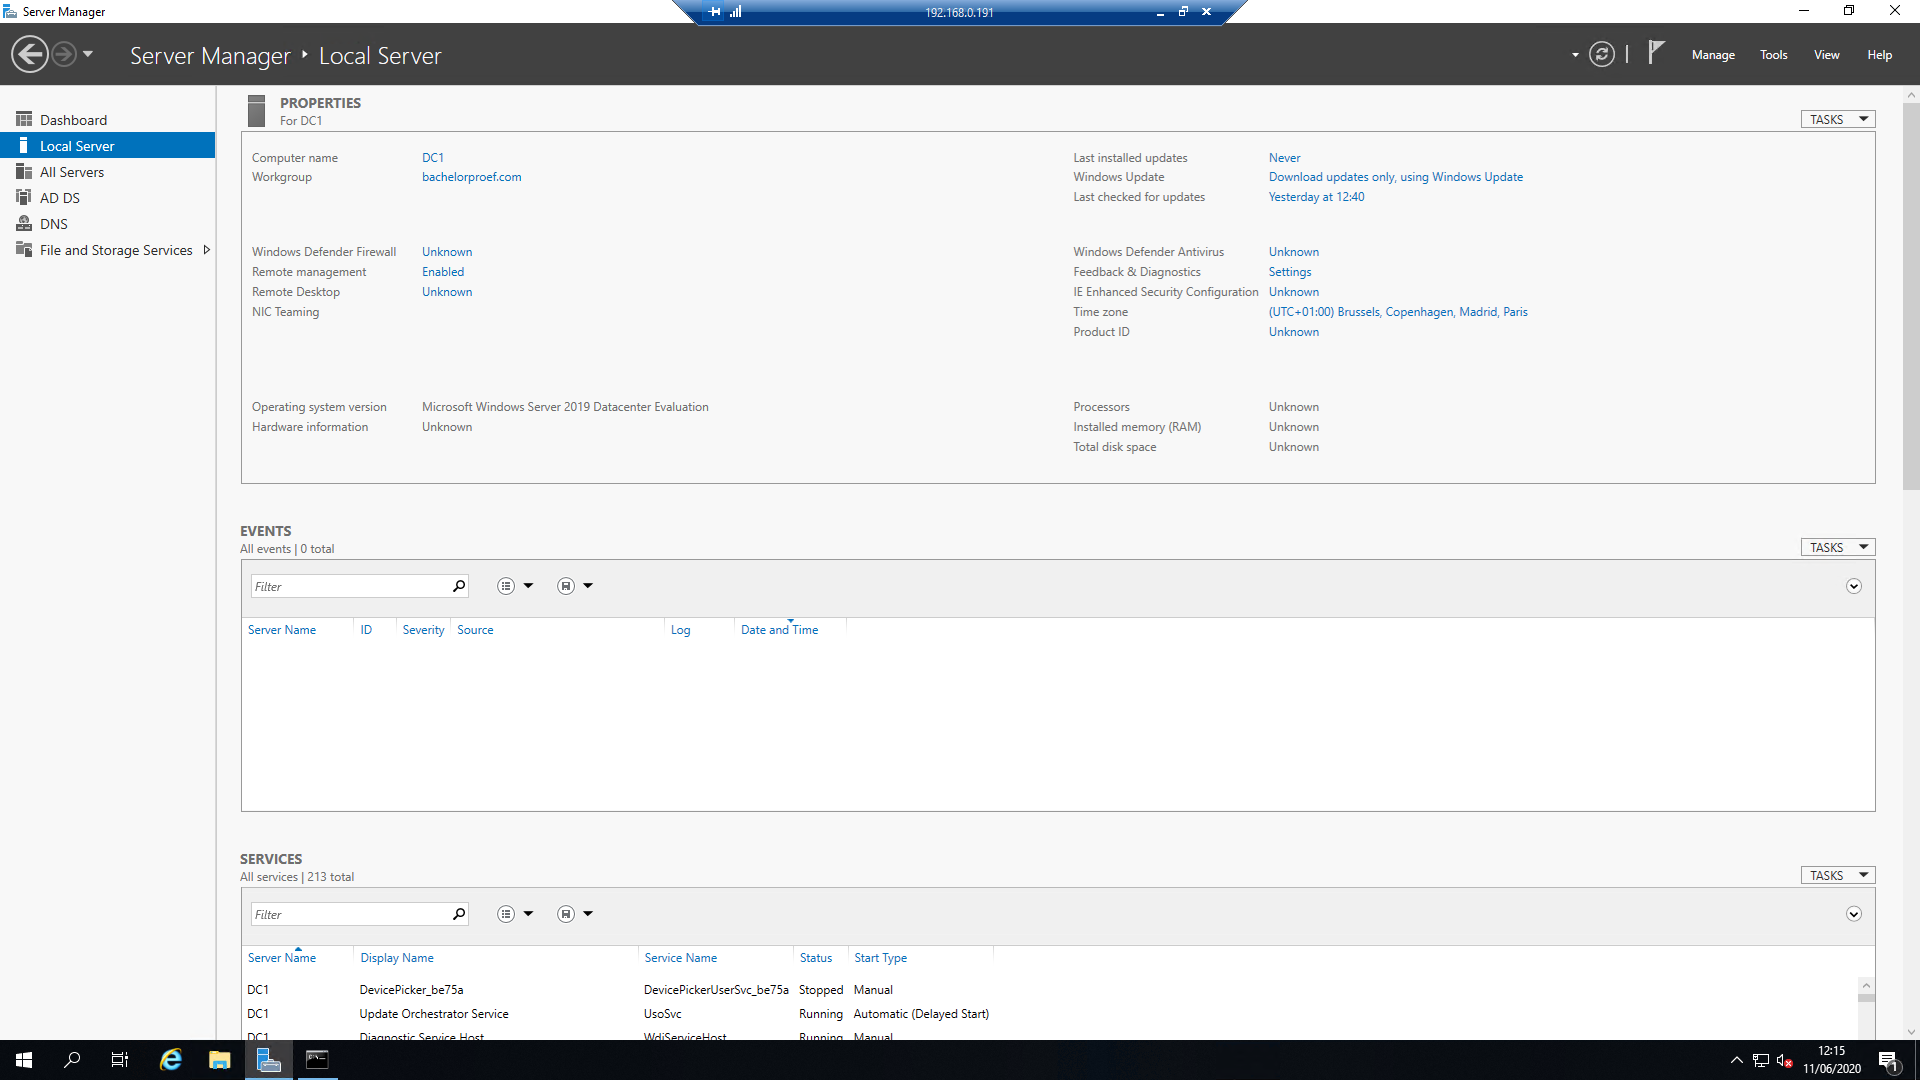
\includegraphics[width=0.6\textwidth]{WindowsHome.png}
	\caption{Deze afbeelding heeft de GUI van Windows server 2019 datacenter weer. }
\end{figure}

\subsubsection{Pfsense}
De Pfsense virtuele machine verwijst naar de virtuele router of firewall. Deze virtuele router maakt communicatie met het afgezonderd netwerk mogelijk. Zoals eerder vermeld werd deze pfsense machine gebruikt  als gateway voor alle vlan’s en alle componenten achterliggend de Cisco switch.
\newline
\newline
Om dit systeem te contacteren, werd het ‘Hypertext Transfer Protocol (HTTP)’ gebruikt met het Internet Protocol (IP) adres van dit systeem. M.a.w. werd er gesurfd naar het 'http://192.168.17.1/'.
\newline
\newline
Dit systeem werd geïnstalleerd op een FreeBSD distributie of Free Berkeley Software Distribution, waar volgende specificaties voor werd vrijgemaakt: 

\begin{itemize}
	\item Geheugen: 4 GB Random Access Memory
	\item Opslag: 25 GB
	\item CPU: 4 cores
	\item Netwerk adapter: Cisco\textunderscore netwerk
\end{itemize}
De installatie van Pfsense werd mogelijk gemaakt door \cite{Pfsense_InstallationGuide}.

\begin{figure}[H]
	\centering
	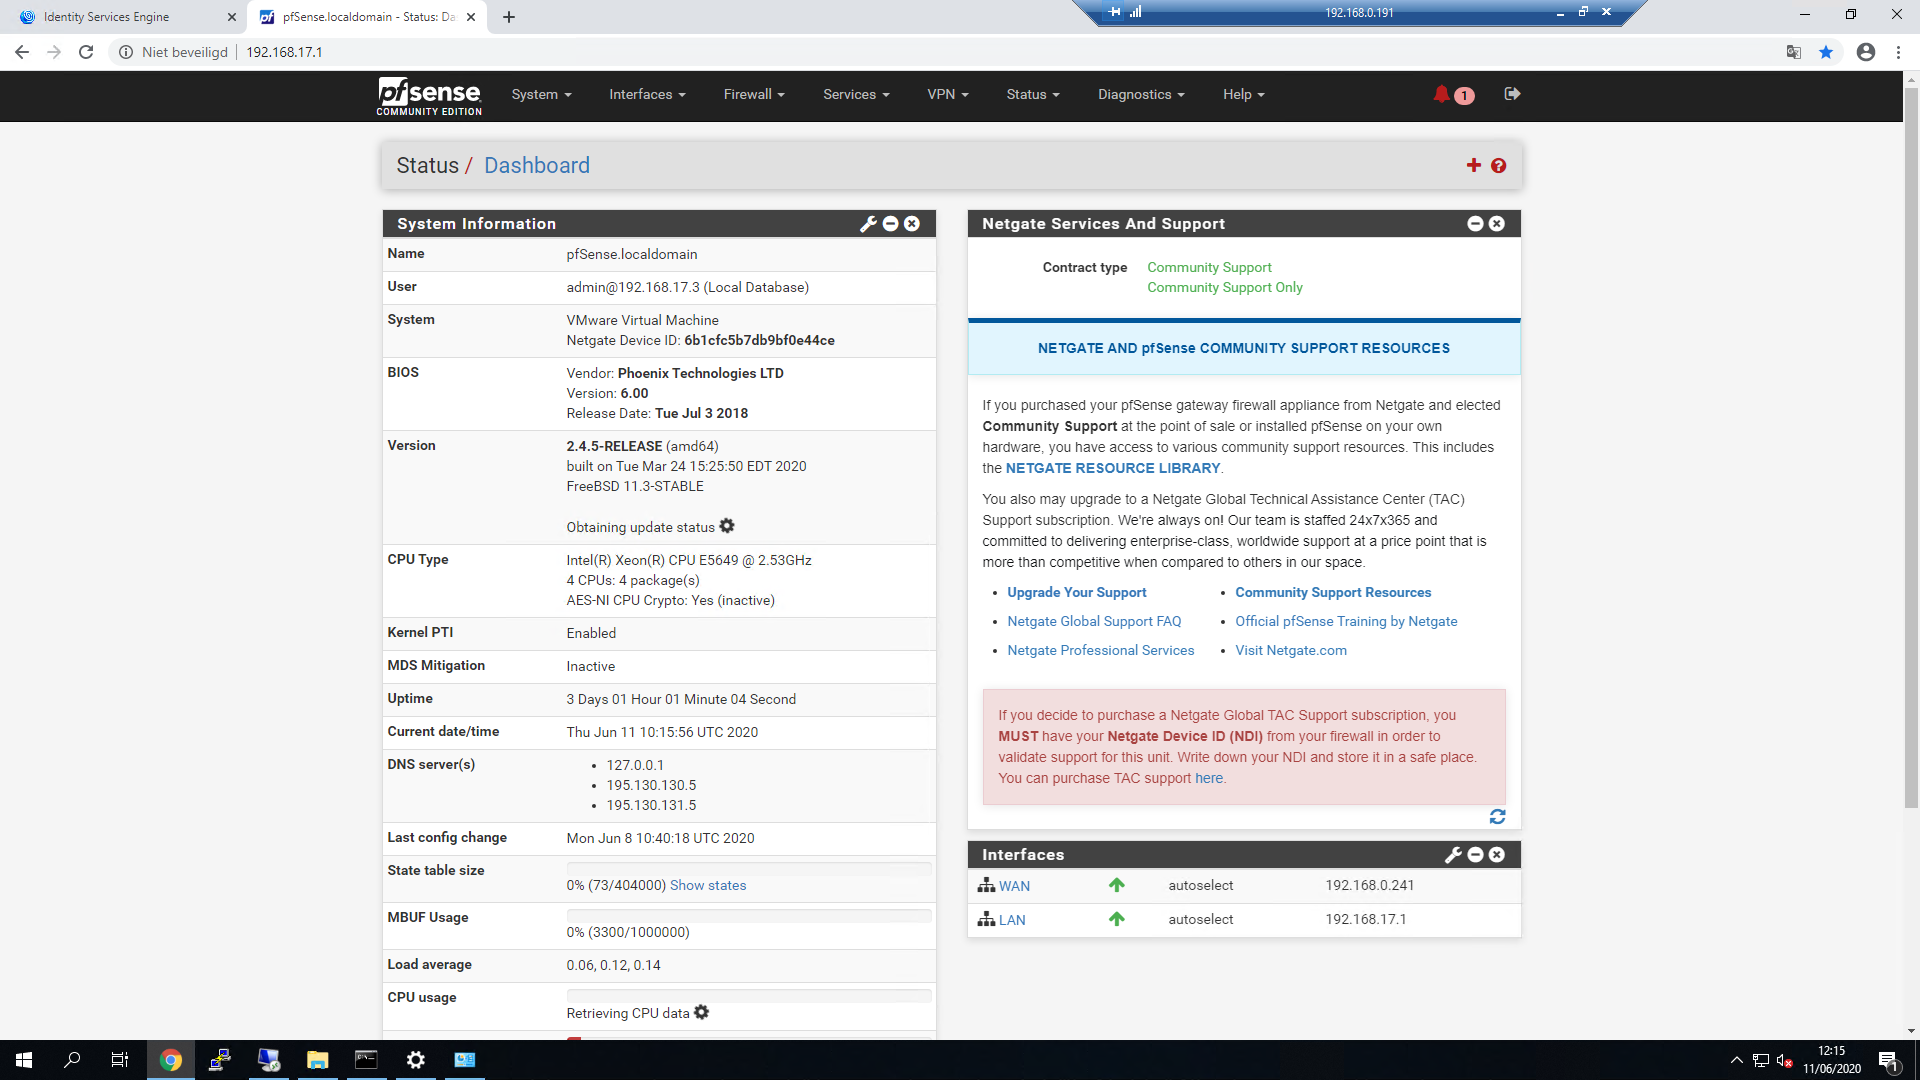
\includegraphics[width=0.6\textwidth]{PfsenseHome.png}
	\caption{Deze afbeelding heeft de GUI van Pfsense weer. }
\end{figure}

\subsubsection{Jumphost}
TO DO!

\begin{itemize}
	\item Geheugen: 16 GB Random Access Memory
	\item Opslag: 126 GB
	\item CPU: 20 cores
	\item Netwerk adapter 1: Cisco\textunderscore netwerk
	\item Netwerk adapter 2: Cisco\textunderscore netwerk
\end{itemize}

De installatie van Pfsense werd mogelijk gemaakt door \cite{Pfsense_InstallationGuide}.

\begin{figure}[H]
	\centering
	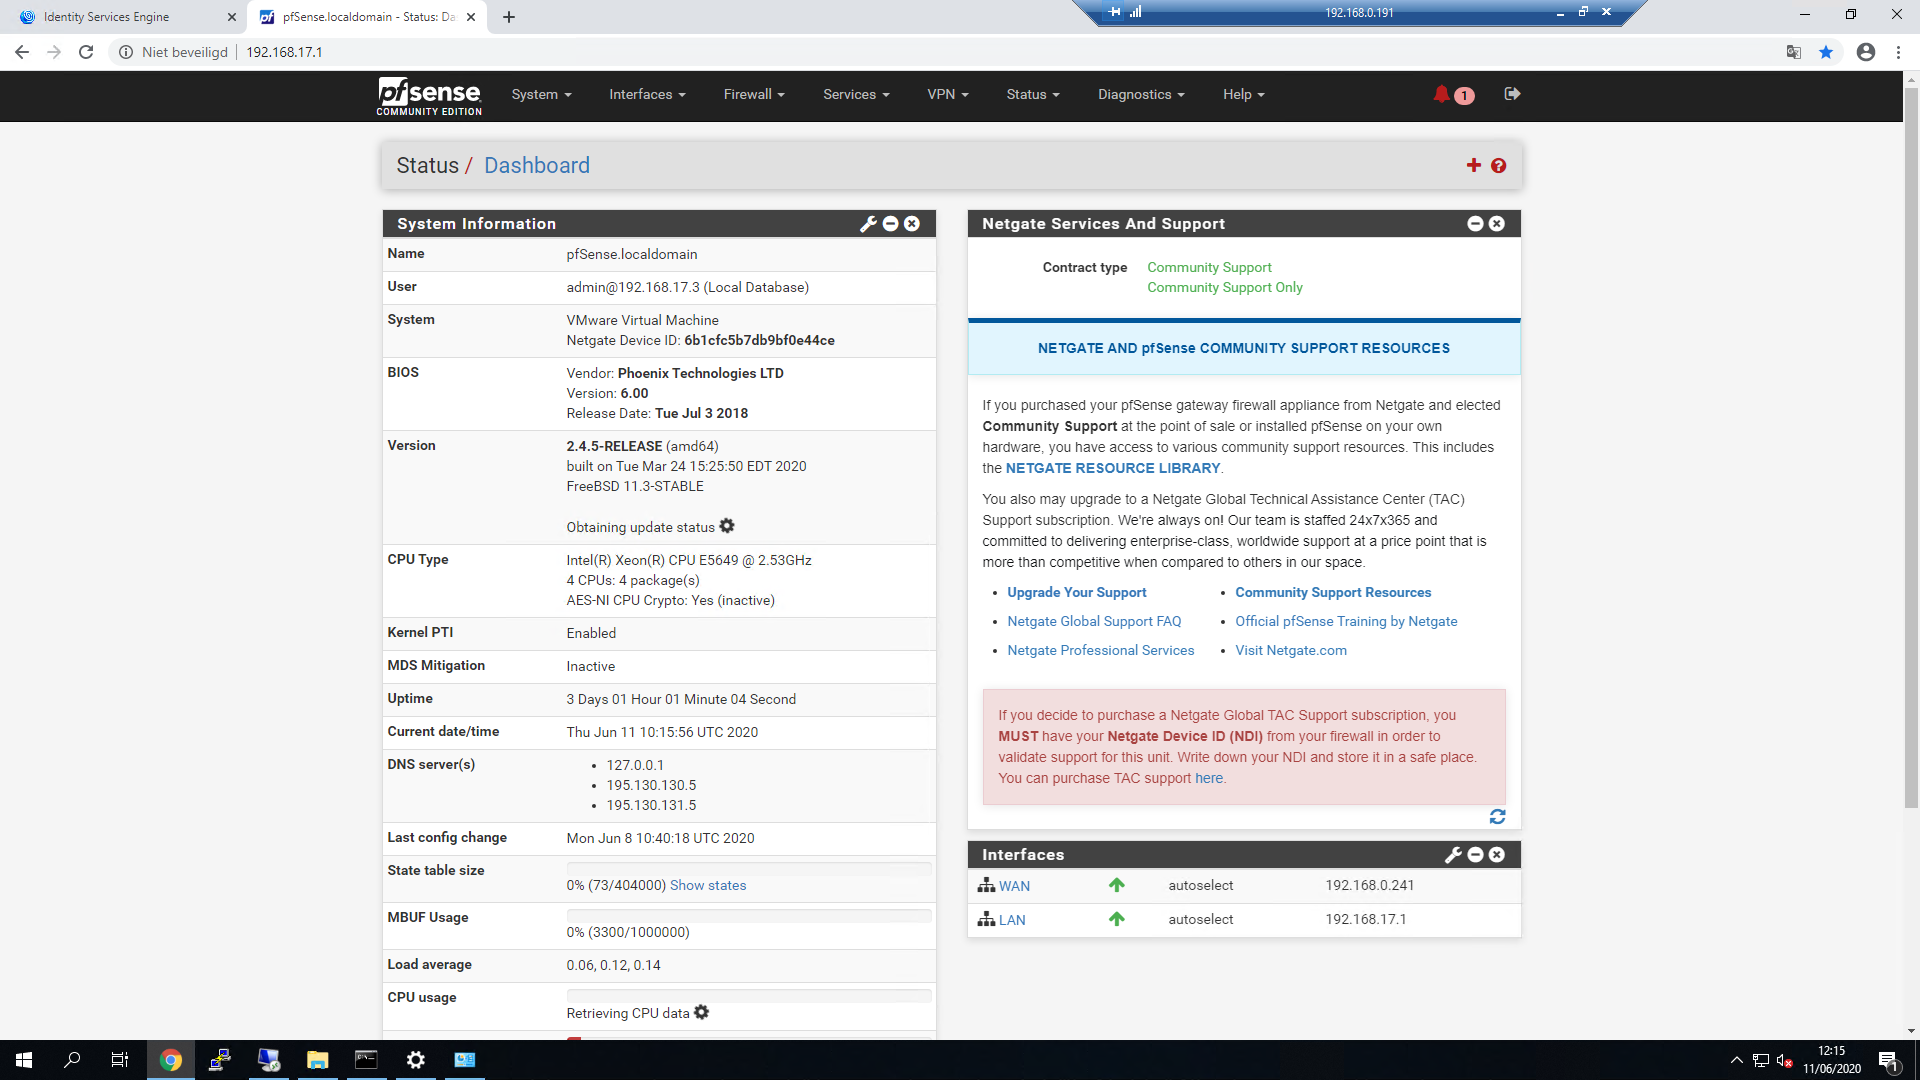
\includegraphics[width=0.7\textwidth]{PfsenseHome.png}
	\caption{Figuur 4.8 heeft de GUI van Pfsense weer. }
\end{figure}

\subsection{Begrippen}
\subsubitem{Telenet Access Point}
\newline
Een Access point is een draadloze server die gegevens verzendt via radio golven in middel van een antenne. Deze gegevens worden ontvangen via het bedrage UTP netwerk waarbij deze “server” is op aan gesloten.
\subsubitem{Telenet Modem}
\newline
Een modem is een toestel die informatie van uw internetprovider ontvangt via een telefoonlijn, glasvezelkabel of coaxkabel in de woning en converteert dit naar een digitaal signaal.
\subsubitem{Coax kabel}
\newline
Een Coax kabel een twee polige kabel die instaat voor het overdragen van beeld en geluid. Deze signalen treden gemakkelijker binnen, waarbij het signaal op korte afstanden snel zwak wordt. 
\subsubitem{Virtual local area network}
\newline
Dit is een type virtueel network dat gerealiseerd wordt op de datalinklaag. Dit bestaat uit een groep eindstations en switches die logisch gezien één enkel gemeenschappelijk local area network (LAN) vormen.

\begin{figure}[H]
	\centering
	\subfloat{{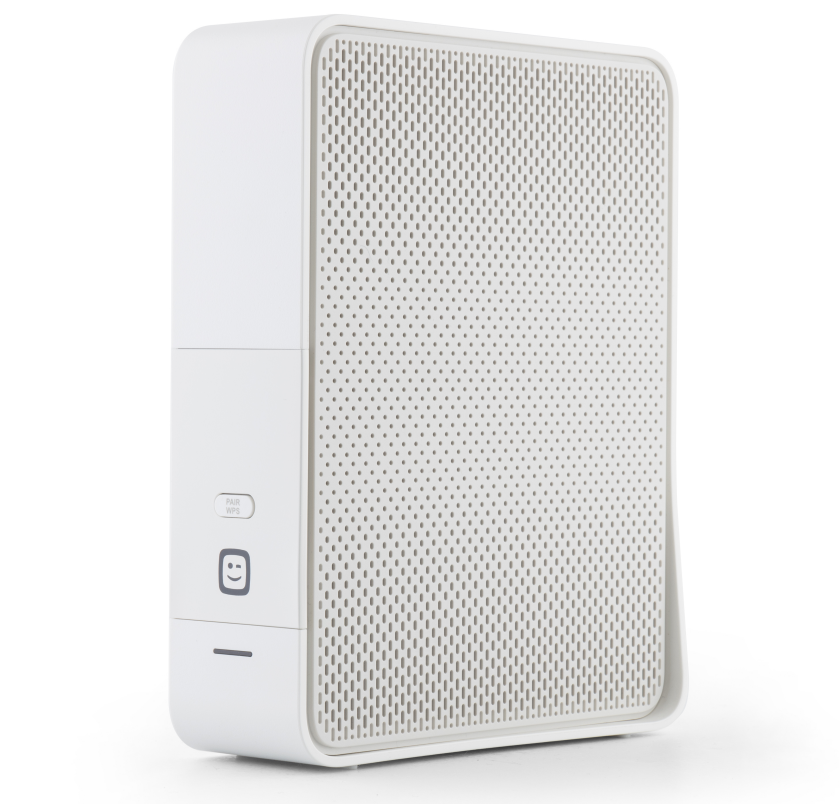
\includegraphics[width=5cm]{TelenetAP.png} }}%
	\qquad
	\subfloat{{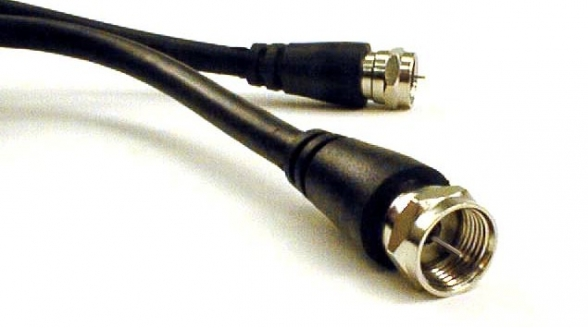
\includegraphics[width=5cm]{Coaxkabel.png} }}%
	\caption{De foto aan de linkerkant is een voorbeeld van een Telenet access point. De foto aan de rechterkant is een voorbeeld van een Coaxkabel.}%
	\label{fig:example}%
\end{figure}
\section{Cisco Identity Services Engine enquête}
Om een link te leggen met de resultaten van de uitgevoerde testen, werd een enquête of een formulier opstelt. Deze enquête is als onderliggende basis gebruikt bij de analyse van de resultaten die verkregen werden door de fysieke testen. Zoals in vorige hoofdstukken vermeld, is deze enquête een opiniepeiling. Waarbij een aantal vragen gesteld zijn aan personen die reeds gekend zijn met Cisco Identity Services Engine. Hierdoor is de doelgroep van deze enquête beperkt tot de Cisco Identity Services Engine specialisten.
\newline
\newline
Deze enquête is publiekelijk gemaakt via LinkedIn en via E-mail. Linkedin is een online sociaal netwerk dat is opgericht voor Vakmensen, die ongeveer 610 miljoen geregistreerden telt. Omdat deze enquête publiekelijk werd gemaakt op \cite{LinkedIn}, bevat dit formulier een aantal ‘failsave’ vragen. Deze ‘failsave’ vragen zijn bedoelt wanneer niet Cisco Identity Services Engine specialisten de enquête proberen in te vullen. Met als gevolg dat de kans op onjuiste ingevuld antwoorden verkleind werd.
\newline
\newline
Dit formulier of enquête werd mogelijk gemaakt door Microsoft en Hogeschool Gent. Elke student heeft recht op een gelicentieerd Office 365 pakket gedurende zijn opleidingstraject. Het programma in kwestie noemt men \cite{MicrosoftForms} dat inbegrepen is in het Microsoft Office 365 pakket.
\newline
\newline
Een overzicht van de vragen die gesteld werden tijdens de enquête is terug te vinden in \ref{ch:Resultaten_enquête}. Bij elke vraag is steeds een klein woordje uitleg gegeven. Idem zoals de mogelijke antwoorden en eventuele doorverwijzingen naar andere vragen.

